\chapter{IPv4 (Internet Protocol Version 4)}
Eine IPv4-Adresse ist eine 32-Bit Zahl. Es gibt also $2^{32}$ $\approx$ 4,3 Milliarden IPv4-Adressen.

\begin{table}[H]
	\begin{tabular}{c|c|c|c}
		 \multicolumn{4}{l}{\textbf{Bsp:}} \\
		11000000 & 10101000 & 00001010 & 00001010 \\
		192 & 168 & 10 & 10 \\
		 \multicolumn{4}{l}{$\rightarrow$ 192.168.10.10} \\
	\end{tabular}
\end{table}
\subsection*{Schreibweise:}
Die IPv4-Adresse wird in Dotted Decimal Notation geschrieben. Die IP-Adresse wird in 8-Bit Blöcke (Oktetten) geteilt, dezimal übersetzt und durch Punkte getrennt.

\subsection*{Verwendung}
Jedes Gerät soll durch eine Adresse (IP-Adresse) eindeutig identifiziert werden. Zusätzlich sollten auch Gruppen (Netze) von Computern erstellt werden (mit Subnetzmasken). Ein Gerät mit IP-Adresse nennt man Host.

\subsection*{Subnetmask}
Ist eine 32-Bit Zahl, die in Dotted Deicmal Notation beschrieben wird. Es kommen zuerst alles Einsen und nach der ersten Null nur noch Nullen. 

\subsubsection*{Typische Subnetmasken}
\begin{table}[H]
	\begin{tabular}{c|c|c}
%		\multicolumn{3}{l}{\textbf{Typische Subnetmasken:}} \\
		& Präfix & Hosts \\
		\hline
		255.0.0.0 & 8 & $2^{24}$ - 2 = 16.777.214 \\
		\hline
		255.255.0.0 & 16 & $2^{16}$ - 2 = 65.534 \\
		\hline
		255.255.255.0 & 24 & $2^{8}$ - 2 = 254
	\end{tabular}
\end{table}
\begin{table}[H]
	\begin{tabular}{cc|cc}
		\multicolumn{4}{l}{\textbf{Bsp:}} \\
		\multicolumn{2}{c}{Telefonnummer} & \multicolumn{2}{c}{IP-Adresse} \\
		+43 664 & 123456 & 172.16. & 20.25 \\
		Netz & einzigartig & 255.255. & 0.0 \\
		 & & Netzteil & Hostteil
	\end{tabular}
\end{table}
Die Subnetzmaske trennt die IP-Adresse in Netzteil und Hostteil. IP-Adresse und Subnetzmaske gehören immer zusammen.

1) 2 IP-Adressen im gleichen Netz \\
10.10.226.120 / 24 \\
10.10.226.80 / 24 \\

2) 2 IP-Adressen nicht im gleichen Netz \\
11.40.30.124 / 24 \\
14.8.50.100 / 24 \\

\begin{table}[H]
	\begin{tabular}{ll}
		\multicolumn{2}{l}{3) Anzahl der Hosts} \\
		$2^{8} - 2$ & 10.10.226.0 (Netzadresse)\\
		& 10.10.226.255 (Broadcastadresse)\\
	\end{tabular}
\end{table}

192.168.20.100 / 8 \\
Netz:  192.0.0.0 \\
Broad: 192.255.255.255


\chapter{Netzwerke im Alltag und Grundbegriffe}
\subsection*{Netzwerk Komponenten}
\begin{itemize}
	\item Endgeräte (PC, Handy, Uhr, TV, Server,...)
	\item Intermediary Devices (Router, Repeater, Switch, Hub, Access Point)
	\item Übertragungsmedien (Drahtlos, Kupfer, Glasfaser)
\end{itemize}

\subsection*{Host-Aufgaben}
\begin{itemize}
	\item Client-Server-Modell
	\item Peer-to-Peer Modell
	\item[] \begin{tabbing}
		+ Komplexität ~~~~~~~~~~~~~~~~~~ \= - Security\\
		+ Leichter zum Aufsetzen ~~~~ \= - Erweiterbarkeit\\
	\end{tabbing}
\end{itemize}

\subsection*{Netzwerk Dokumentation}
\begin{itemize}
	\item Physische Topologie (Räume, ...)
	\item Logische Topologie (Netze, ...)
\end{itemize}

\subsection*{Netzwerke nach Größe}
\begin{itemize}
	\item SOHO ... small office home office
	\item LAN ... local area network
	\item MAN ... metropolitan area network
	\item WAN ... wide area network
	\item Internet
\end{itemize}

\subsection*{Netzwerke nach Funktion}
\begin{itemize}
	\item SAN ... storage area network
	\item Intranet, Extranet
\end{itemize}

\subsection*{Internetzugang}
\begin{itemize}
	\item Kabel (Glasfaser)
	\item DSL / Dial Up
	\item Mobilfunknetz
	\item Satellit
\end{itemize}

\subsection*{Trends}
\begin{itemize}
	\item Video / Streaming
	\item Cloud
	\item Drahtlos (5G)
	\item BYOD (bring your own device)
	\item Online Collaboration
	\item Powerline Method
\end{itemize}

\subsection*{Netzwerkarchitektur}
\begin{itemize}
	\item Quality of Service QoS
	\item Erweiterbarkeit
	\item Security
	\item Fehlertoleranz
\end{itemize}

\subsection*{Security}
\begin{itemize}
	\item Ransomware
	\item DoS / DDoS
	\item Virus, Wurm, Trojaner
	\item Social Engineering
	\item Zero-Day-Attack
\end{itemize}

\section{Referenzmodell (OSI und TCP/IP)}
\begin{center}
	\begin{tabular}{|cl|l|c|}
		\hline
		\multicolumn{2}{|c|}{OSI} & \multicolumn{1}{c|}{Protokolle} & TCP/IP \\ \hline
		\multicolumn{1}{|c|}{7} & Application Layer & HTTPS, FTP, Telnet, SSH & \multirow{3}{*}{Application Layer} \\ \cline{1-3}
		\multicolumn{1}{|c|}{6} & Presentation Layer & POP, SMTP, IMAP &  \\ \cline{1-3}
		\multicolumn{1}{|c|}{5} & Session Layer & DHCP, NTP, DNS &  \\ \hline
		\multicolumn{1}{|c|}{4} & Transport Layer & TCP, UDP & Transport Layer \\ \hline
		\multicolumn{1}{|c|}{3} & Netzwerk Layer & IP, ICMP; OSPF, BGP, RIP & Internet Layer \\ \hline
		\multicolumn{1}{|c|}{2} & Data Link Layer & \multirow{2}{*}{Wifi, Ethernet, ARP} & \multirow{2}{*}{Network Access Layer} \\ \cline{1-2}
		\multicolumn{1}{|c|}{1} & Physical Layer &  &  \\ \hline
	\end{tabular}
\end{center}

\begin{figure}[H]
	\centering
	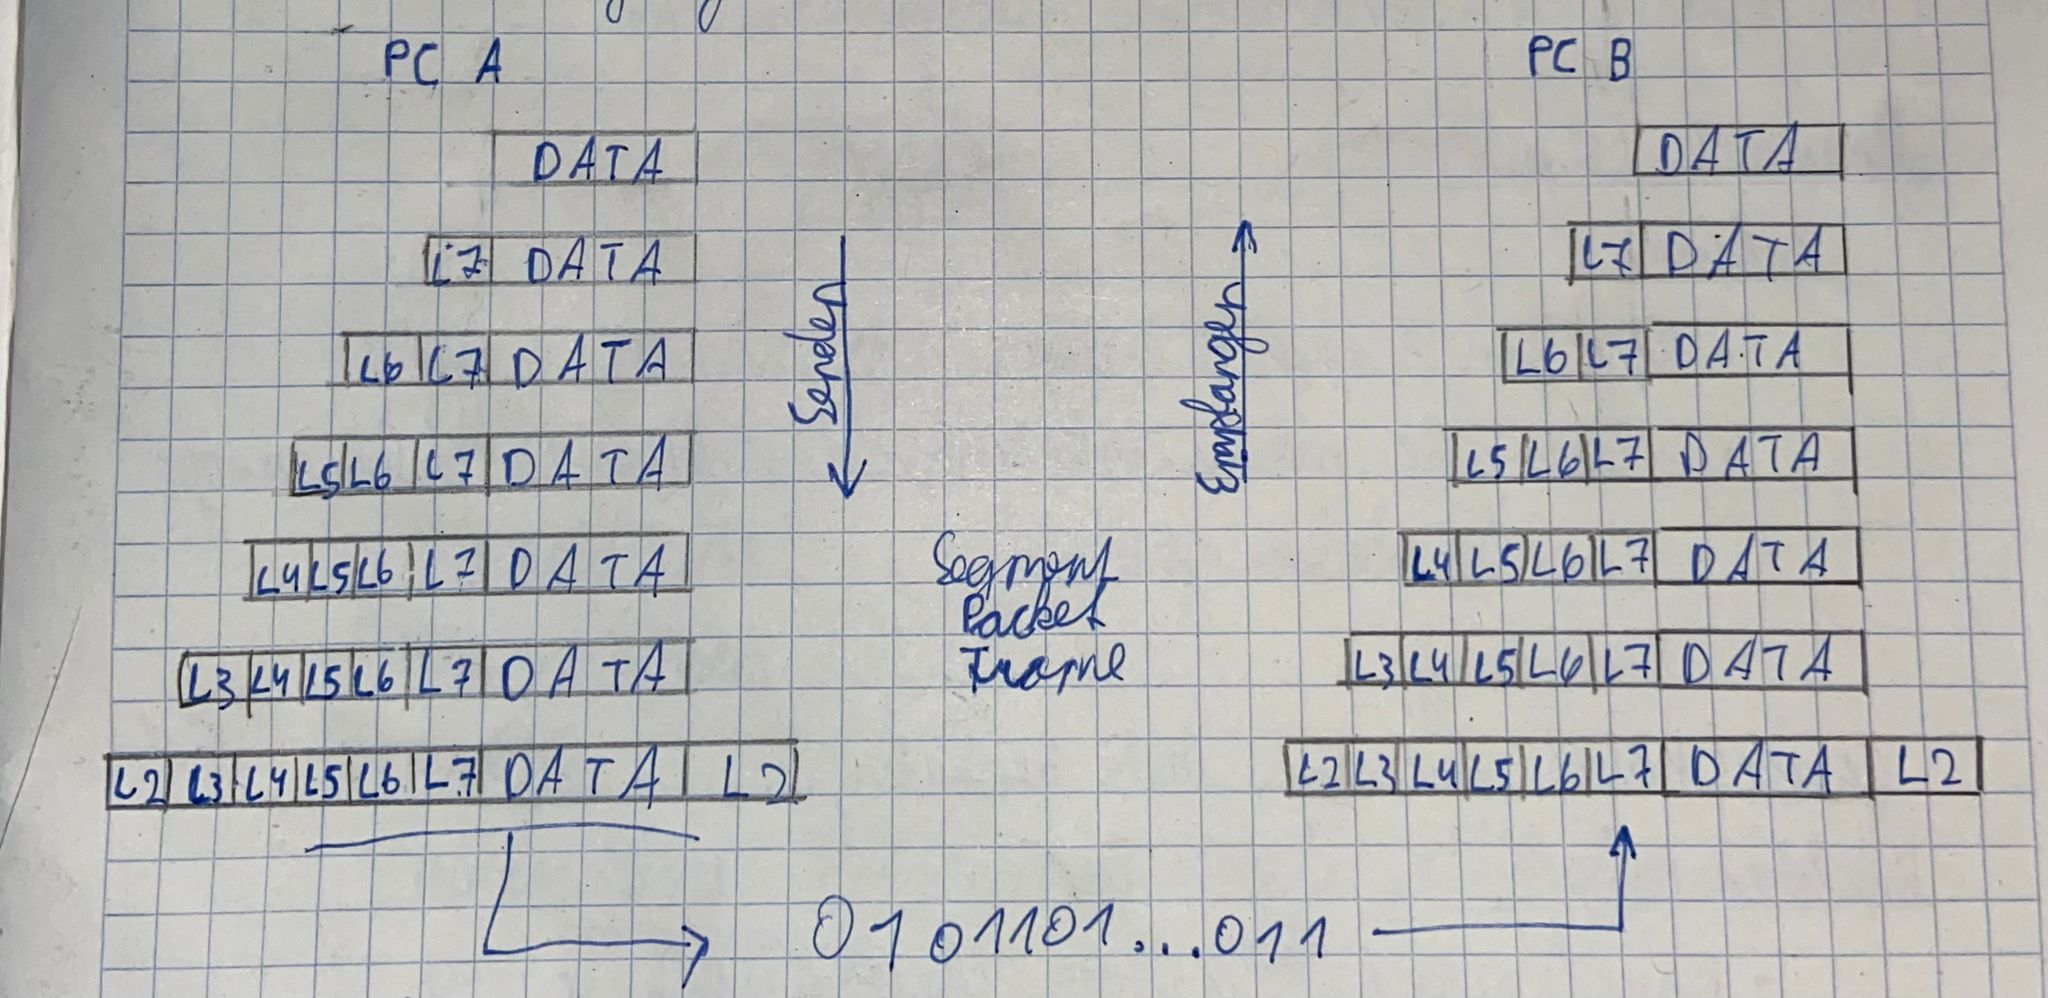
\includegraphics[width=0.9\linewidth]{figures/datenuber.jpeg}
	\caption{OSI-Modell Datenübertragung}
\end{figure}

\textbf{Layer 1 (Physical):} Bits übertragen \\
\textbf{Layer 2 (Data Link):} Lokale Adressierung, Fehlererkennung \\
\textbf{Layer 3 (Network):} Globale Adressierung, Routing \\
\textbf{Layer 4 (Transport):} Datenpaketzuordnung, Segmentierung, Datenfluss steuern \\
\textbf{Layer 5 (Session):} Session Verwalten, Verschlüsselung \\
\textbf{Layer 6 (Presentation):} Darstellung der Daten \\
\textbf{Layer 7 (Application):} Funktionen für die Application \\

\subsection*{Cisco CLI}
\begin{figure}[H]
	\centering
	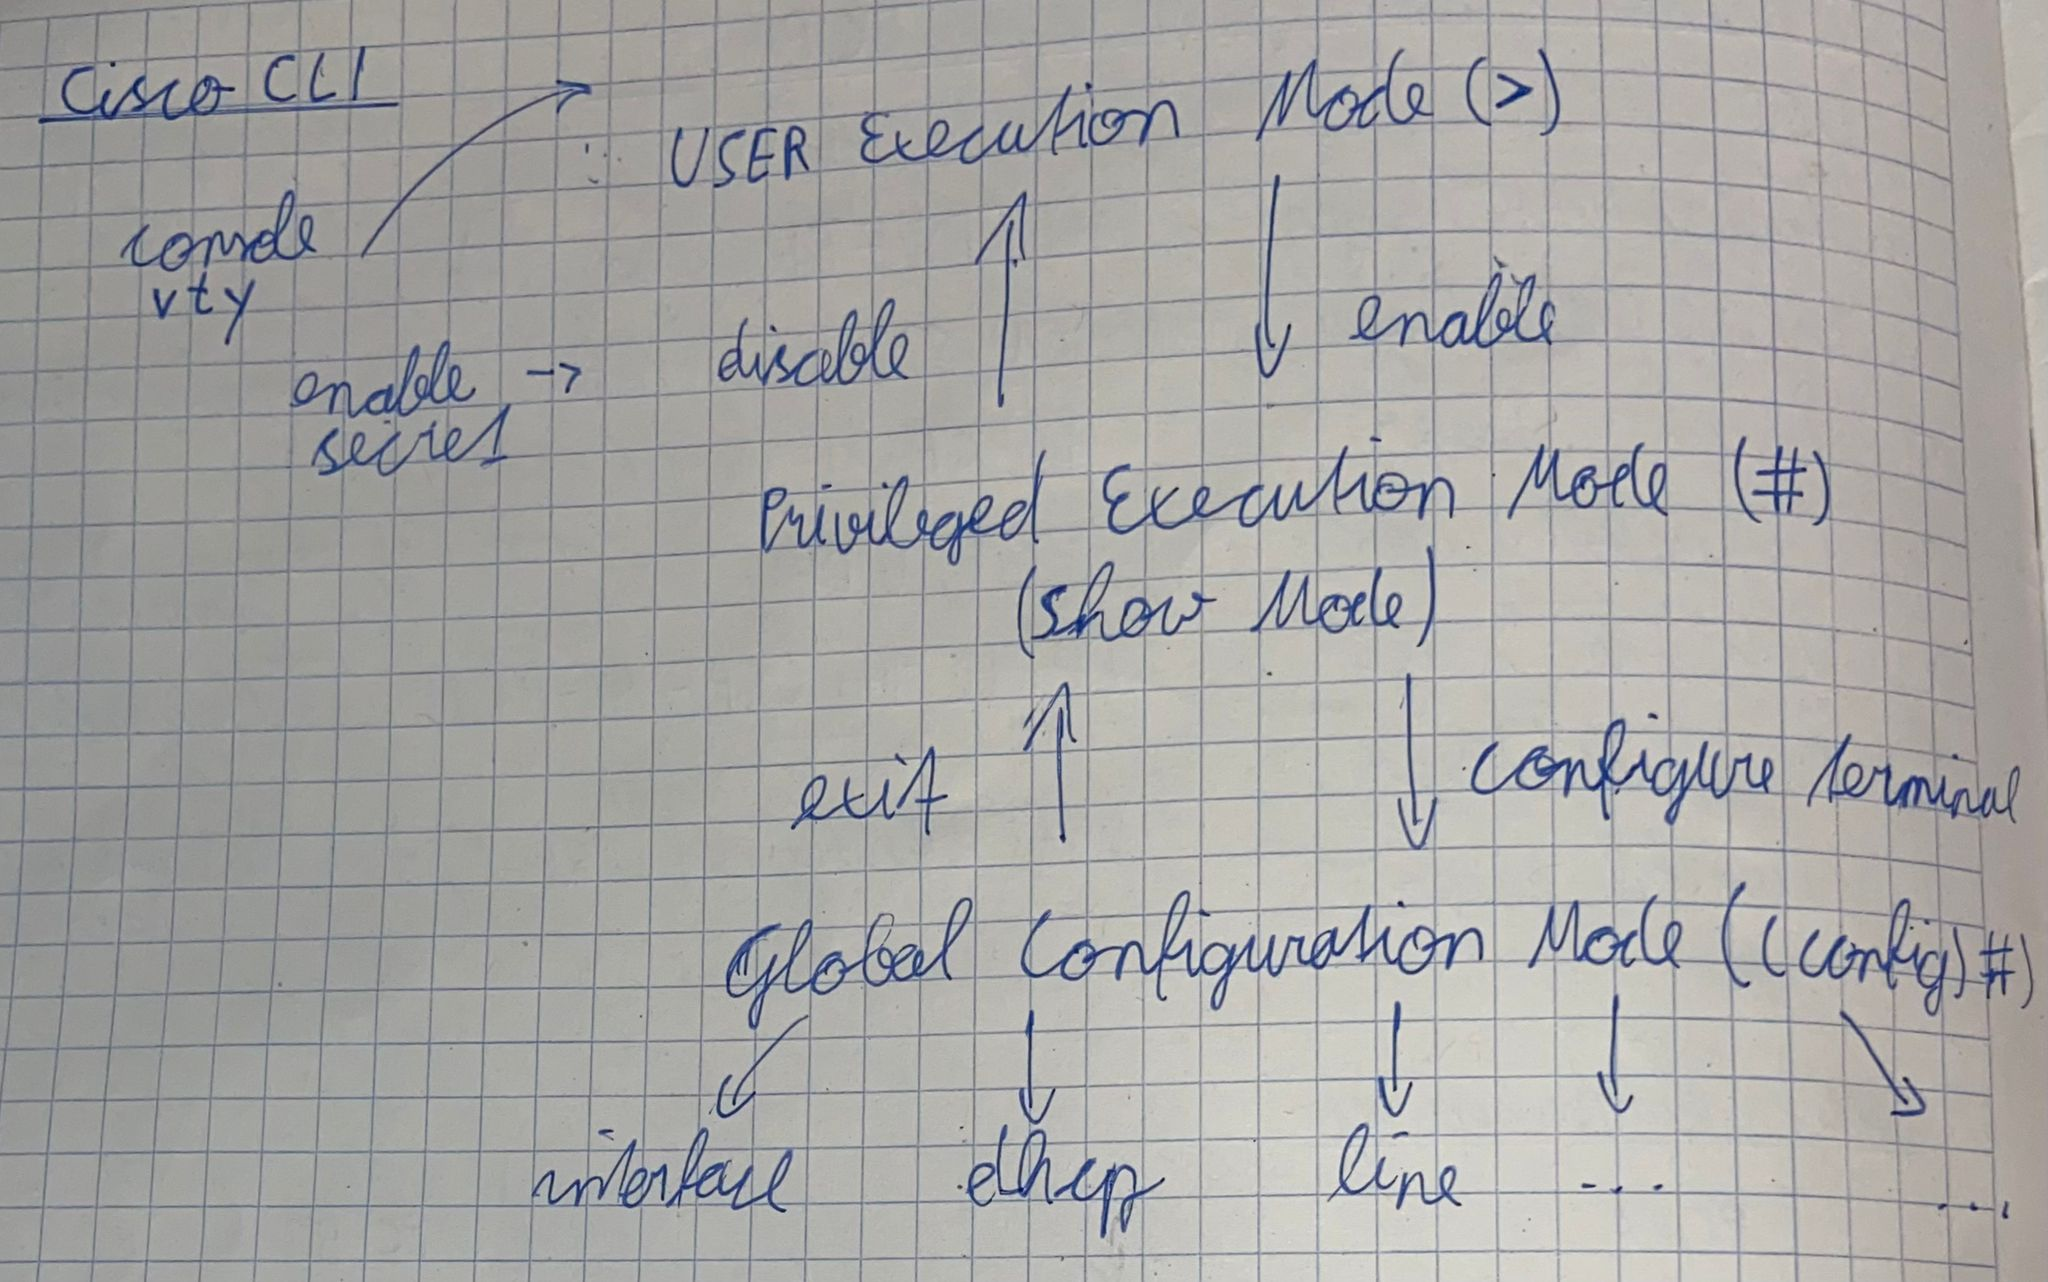
\includegraphics[width=0.9\linewidth]{figures/ciscocli.jpeg}
	\caption{Cisco CLI}
\end{figure}